\documentclass[../Report.tex]{subfiles}


\begin{document}


\chapter{Einführung}
\label{chap:einfuehrung}
Mit den Barrier Bucket (BB) RF Systemen können am neu entstehenden Synchrotron SIS100 oder im Experimentier Speicherring (ESR) am GSI Helmholtzzentrum viele longitudinale Manipulationen am Teilchenstrahl vor genommen werden. Der dazu benutzte Spannungspuls hat die Form wie in \figref{fig:BB_req} dargestellt. Wenn die Wiederholfrequenz des Spannungspulses gleich der Umlauffrequenz ist, so wird im Phasenraum eine stationäre Potential Barriere erstellt. Wenn die Wiederholfrequenz nicht gleich der Umlauffrequenz ist verschiebt sich die Potential Barriere im Phasenraum und es entstehen Bunches mit unterschiedlicher Länge. \\ Der Anspruch an diese Systeme liegt darin eine hohe Qualität des Impulses am Gap der Kavität zu erzeugen. Um sogenannte Microbunches zu verhindern müssen die Nachschwinger nach dem Einzelsinus kleiner als 2,5\% von $\hat{U}_{BB}$ sein.
\begin{figure}[H]
  \centering
  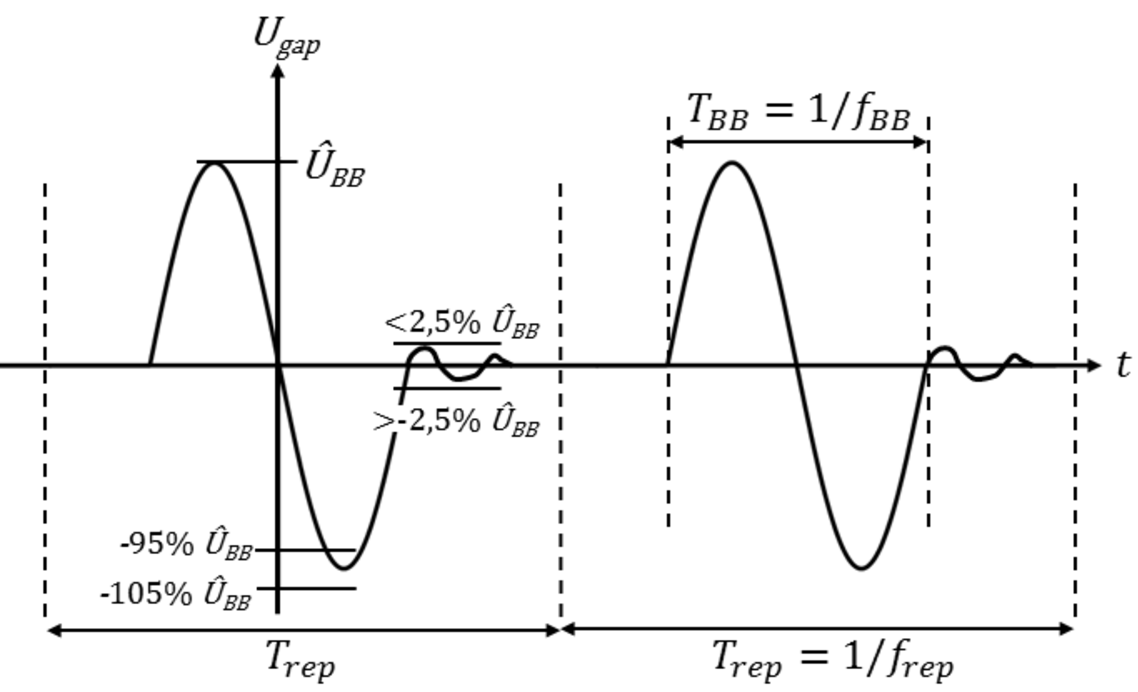
\includegraphics[width=0.7\textwidth]{images/eps/BB_req.pdf}
  \caption{Ausgangssignal}
  \label{fig:BB_req}
\end{figure}
SCHÖNHEITSFEHLER HIER Dabei benutzen wir im Folgenden $f_{rep}$ für die Wiederholfrequenz des Spannungssignals und die Barrier Bucket Frequenz $f_{BB}$ bestimmt die Breite der Potential Barriere. Für unsere Messungen haben wir ${f_{rep} = 900 \si{\kilo \hertz}}$ und ${f_{BB} = 5 \si{\mega \hertz}}$ verwendet.
\section[Modell und Konvention]{Versuchsaufbau und Modell}
\label{sec:einf.modell_BB}
Der Prototyp des ESR BB besteht aus einem Funktionsgenerator (Keysight 3600A series 2-channel AWG), einem Verstärker (AR1000A225) und der Breitband Ringkern Kavität. Der Versuchsaufbau ist in \figref{fig:Aufbau} gezeigt.\\Dabei kann angenommen werden, dass sich das System bis $\hat{U}_{BB} = 550V$ annähernd linear verhält und durch die Übertragungsfunktion $\Hcompl \ofomega$ beschrieben werden kann. Eine mathematische Modellierung ist ebenfalls in \figref{fig:Aufbau} gegeben, bei der zur linearen Übertragungsfunktion $\Hcompl \ofomega$ noch eine nichtlineare Kennlinie $K$ enthalten ist.
\begin{figure}[H]
	\centering
	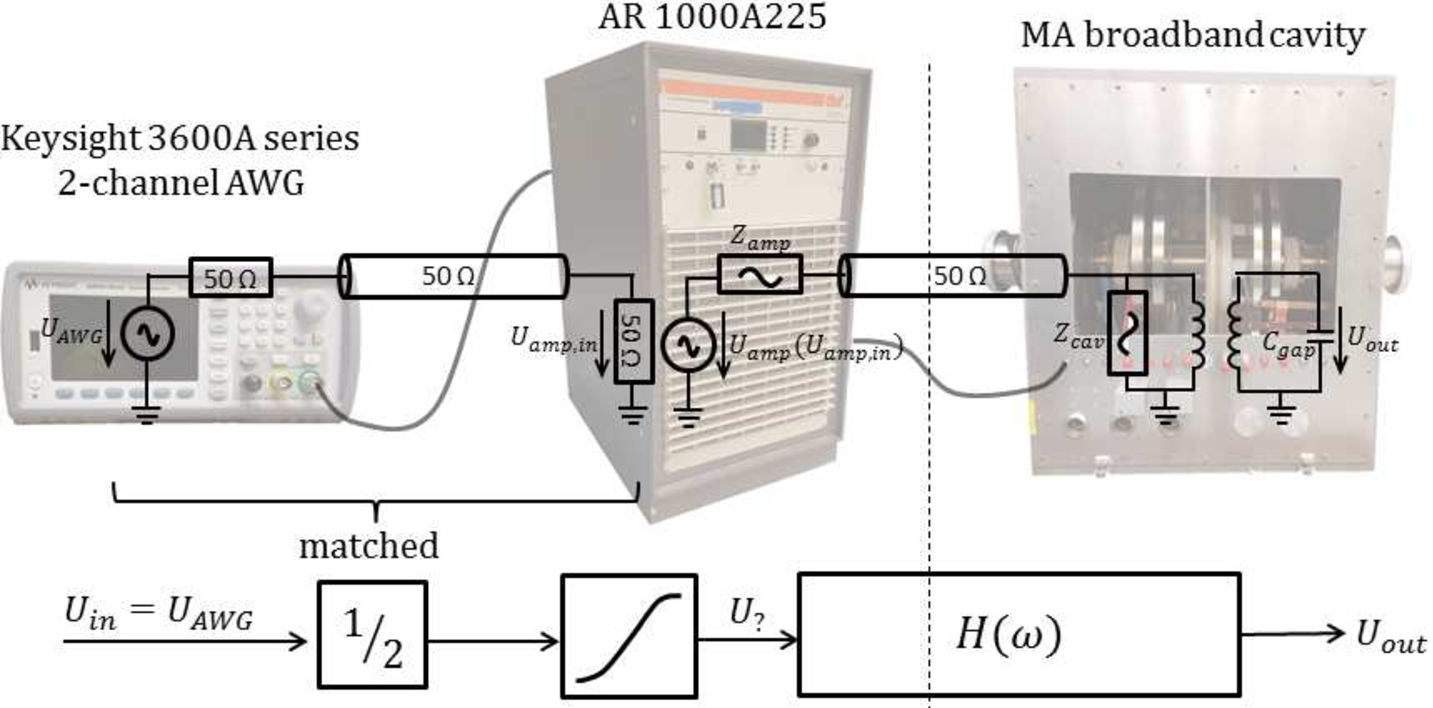
\includegraphics[width=0.7\textwidth]{images/eps/Aufbau.pdf}
	\caption{Versuchsaufbau und Modell}
  	\label{fig:Aufbau}
\end{figure}
\subsection{Hammerstein Modell}
\label{subsec:einf.modell_BB.hammerstein}
In \figref{fig:Hammerstein} sind alle von uns verwendeten Größen dargestellt. $U_{in}$ ist die Eingangsspannung vom Funktionsgenerator. Dabei stellt der erste Block die nichtlineare Modellierung dar. Die Größe $U_{?}$ ist eine rein virtuelle Größe und kann wie in \ref{eq:Uquest} berechnet werden oder über die Inverse der Übertragungsfunktion $\underline{H}^{-1} \ofomega$ von $U_{out}$ zurückgerechnet werden. Bei der Potenzreihe hatte $N = 3$ in der Implementierung in MATLAB schon gute Ergebnisse geliefert und wurde von uns auch weiterhin so verwendet.
\begin{figure}[H]
	\centering
	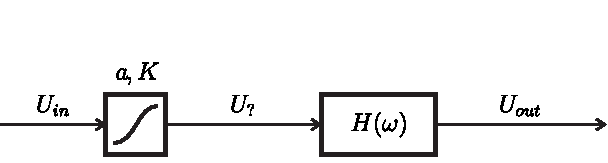
\includegraphics[width=0.5\textwidth]{images/eps/Hammerstein.pdf}
	\caption{Hammerstein Modell}
  	\label{fig:Hammerstein}
\end{figure}
\begin{align}
	U_?(t)=\sum_{n=1}^N \, a_n \, \left[ U_{in}(t) \right]^n
	\label{eq:Uquest}
\end{align}
\section{Motivation}
\label{sec:einf.motivation}
Warum haben wir unser Design so gewählt?...

\section{Aufgabenstellung}
\label{sec:einf.problem}
Im Rahmen unseres Projektseminar sollte eine iterative Optimierung der Vorverzerrung auf Basis einer Hammersteinmodellierung in Python implementiert werden. Dabei sollte die Weiterentwicklung des Python-Tools im Vordergrund stehen.
\end{document}